\chapter{Extension to Multiple Particles}

We now present an extension of this work for draining multiple particles out of a workpiece. The initial adaption to our approach is fairly trivial, but the two heuristics we present shortly afterwards dramatically improve search performance.

\section{Initial Adaption}

Only two elements of our approach need to be modified in order to drain multiple particles out of a workpiece. The first is a modification to the state definition; the state is now a set of settled locations, one for each particle:

\myequation{
  (V_{cc}^{1}, V_{cc}^{2}, V_{cc}^{3}, ... , V_{cc}^{n})
} {
  \label{eq:multipleParticleState}
}

The second modification is to our successor function definition; the successor function now takes in a set of particle locations and produces a set of ``reachable'' states:

\myequation{
  successor((V_{cc}^{1}, V_{cc}^{2}, ... , V_{cc}^{n})^i) = \left \{ (V_{cc}^{1}, V_{cc}^{2}, ... , V_{cc}^{n})^1, (V_{cc}^{1}, V_{cc}^{2}, ... , V_{cc}^{n})^2, ...  \right \}
} {
  \label{eq:successorMultipleParticle}
}

With only these modifications alone, we are now able to search for solutions that drain multiple particles out of the workpiece.

\subsection{Implementation}

These two modifications to our approach result in a fair number of changes in the implementation. One primary implementation difference is that now a given turn must be simulated across all particle locations. This simulation is usually performed by the transition function:

$$
trans(V_{cc}^{i}, turn_{l}) = V_{cc}^j \qquad or \qquad exit
$$

Earlier we had restricted our action space to only turns that produced motion of the particle and kept the particle on the leading edge of the concave vertex.

This leads to four possible scenarios when simulating a turn for a given particle in a concave vertex:

\begin{itemize}
\item The particle is offscreen; a turn does not change this particle's state.
\item The turn results in no motion; any linear combination between $g_{start}$ and $g_{end}$ does not produce motion of the particle.
\item Motion of the particle starts immediately when the turn begins; $g_{start}$ is defined as one of the perpendicular edge vectors, similar to the single-particle simulation.
\item Motion of the particle starts midway through the turn; $g_{start}$ does not produce motion and $g_{end}$ does.
\end{itemize}

The multiple-particle version of the transition function must be much more robust against arbitrary input.

\section{Multiple Particle Time Complexity}

Now that our state is defined as a set of concave vertex locations, the state space is unfortunately exponential in the number of particles, with a base defined as the number of concave vertices in the workpiece:

$$
(num(V_{cc}) + 1)^n
$$

This leads to a time-complexity that is now exponential in the number of concave vertices, rather than linear as in \eqref{eq:bigo}:

\myequation{
O(S \cdot E^2 \cdot V_{cc}^{n})
} {
  \label{eq:bigoTotal}
}

Although we earlier had avoided exponential state spaces and runtimes due to our search formulation, the introduction of multiple particles has yet again vastly expanded our state space.

\section{Search Heuristics}

The one advantage of multiple-particle draining is that it allows for more creativity and flexibility when composing search optimizations.

\subsection{Plan Ranking Heuristic}

The first optimization (and true search heuristic) we implemented was simply a ranking of the partial plans enqueued onto the priority queue during uniform cost search. Rather than ranking only by cost, we also implemented these two optimizations:

\begin{itemize}
\item Always prefer plans with a higher number of exited particles, overriding all else
\item Determine the number of particles in the same location and use this feature to rank plans
\end{itemize}

In practice for our parts, we discovered that ranking plans by

$$
time - 10 \cdot numSame
$$

produced the best mix between optimality of plans and speed of search.

\subsection{Min Pocket Action Space Heuristic}

The second search optimization we present is centered around sampling from the action space. Recall that for a single particle, we define our action space to sample from as a fixed set of $g_{start}$ vectors and a range of $g_{end}$ vectors that produce motion of the particle, as seen in Figure \ref{restriction3} (shown below for convenience).

\begin{figure}[H]
  \centering
    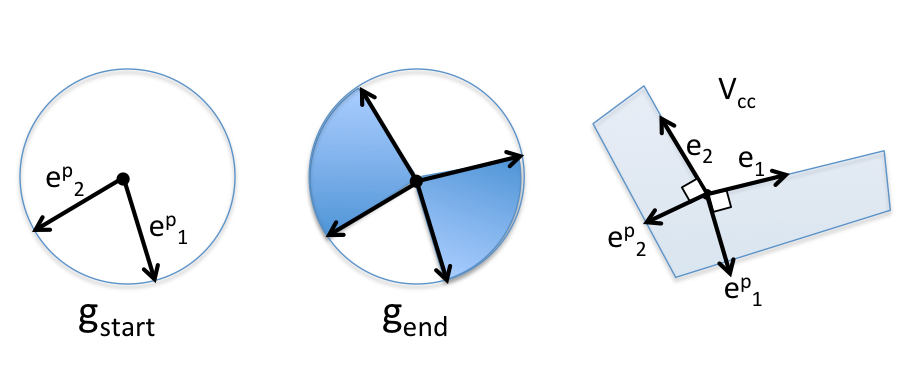
\includegraphics[width=\0.8\linewidth]{figures/restriction3/figure.png}
\end{figure}

% figures


